\chapter{Kern der Arbeit}

\anno{ca. 15-20 Seiten (10)}

% Probleme und die Loesungsansaetze
\section{Probleme}
\label{sec:Probleme}

Der im vorherigen Kapitel betrachtete zeitliche Rahmen, über die Entwicklung von Web Application Firewalls, umfasst mehr als zwanzig Jahre. Ein Zeitraum in dem sich zahlreiche Produkte in diesem Bereich etablierten. Im Anhang finden Sie, beispielsweise, mit der Tabelle~\ref{tab:my_wafwoof} eine (nicht vollständige) Liste von derzeitigen WAF-Produkten verschiedener Hersteller. Über den gesamten Zeitraum haben sich Webtechnologien weiterentwickelt und auch die Art und Weise der Nutzung des Internets änderte sich. Mit der Verbreitung der Smartphones und Sprachassistenten wurden aus einfachen Webangeboten vielschichtige Anwendungen mit verschiedenen möglichen Clientsystemen (\emph{mobile-first-Ansatz}). Serviceorientierte Architekturen, Webservices, Microservices, Künstliche Intelligenz - alles entwickelte sich weiter. Im Bereich der IT-Sicherheit veröffentlichte das \emph{Open Web Application Security Project} 2019 erstmals eine Liste seiner zehn kritischsten Sicherheitsrisiken explizit für den Bereich der \emph{API}s. \emph{ModSecurity} ist immer noch der de-facto-Standart für regelbasierte WAFs und praktisch so gut wie der einzige verbliebene Vertreter der Web Application Firewalls aus dem OpenSource-Bereich. Freie anomaliebasierte Systeme sind so gut wie nicht existent und die privatwirtschaftlichen Akteure lassen sich kaum in die Karten schauen. \\
Mittlerweile sind bereits dreizehn Jahre seit dem Erscheinen des Datensatzes CSIC2010 vergangen und schaut man in die derzeitig vorhandene Literatur scheint auch kein Nachfolger in Sicht. \\\\

\textcolor{bhtGray}{\ding{110} Applebaum über den Datensatz CSIC2010~\cite{Applebaum2021}} Torrano-Giménez et al. provide an HTTP dataset intended to be used for the development and testing of Intrusion Detections Systems and WAFs. ... The dataset has been used extensively by other researchers ... There is still a need for a development of a new dataset as previous datasets had become outdated and did not target real systems. The dataset .. is itself now over 10 years old and targets a bespoke e-commerce system. \\\\

Dennoch ist der Datensatz weiterhin Ausgangsbasis für viele Forschungsvorhaben und praktische Projekte im Bereich der IT-Sicherheit. Im folgenden Kapitel wird daher näher auf den Datensatz CSIC 2010 eingegangen, dessen Aufbau und Verwendung erläutert und es werden mögliche Verbesserungen anhand von praktischen Beispielen vorgeschlagen.
%

\subsection{Aufbau und Format des Datensatzes CSIC2010}
\label{sec:aufbauformat}
% Aufbau /motivation von gimenez

% Aufbau
Der Datensatz besteht aus drei Teildatensätzen. Der erste Teildatensatz ist dabei für die Trainingsphase gedacht und enthält 36000 einzelne HTTP-Anfragen die den normalen bzw. erwünschten Datenverkehr abbilden. Die anderen beiden Teildatensätze sind für die Testphase gedacht. Ein Teildatensatz mit ebenfalls 36000 Anfragen an normalem Datenverkehr und ein Teildatensatz mit über 25000 Anfragen mit Gefährdungspotential (siehe \cite{csic2010}).\\

Die einzelnen Dateneinträge der drei Teildatensätze sind jeweils gleich aufgebaut und beinhalten die in Tabelle~\ref{tab:csicfields} aufgeführten Felder. Das Feld \emph{Payload} ist im Datensatz nicht explizit benannt bzw. auf den ersten Blick nicht ersichtlich, da es je nach HTTP-Methode in den Rohdaten unterschiedlich abgebildet wird. Bei einem \verb=GET=-Request wird die Payload im Query der URL übertragen (siehe \cite{rfc2626} 3.2.2) und bei \verb=POST=-Requests im Request Body. Die Payload enthält im Wesentlichen die eigentlichen Daten und in den meisten Angriffsfällen genau die Anomalien die für einen Angriff verantwortlich sind. Zur Verdeutlichung zeigt Abbildung~\ref{fig:ccex} einen einzelnen Eintrag des Datensatzes \emph{CSIC2010} im Rohformat. Hier handelt es sich um einen \verb=GET=-Request mit den Parametern \emph{id},\emph{nombre}, \emph{precio}, \emph{cantidad} und \emph{B1}. Die einzelnen Dateneinträge des Datensatzes unterscheiden sich jedoch nicht in den übrigen Feldern.\\

Für eine Klassifizierung können bzw. müssen aus den Daten der einzelnen Requests entsprechende Features (\emph{Merkmale~-~individuell messbar}) abgeleitet werden. \emph{Achtung}, Felder und Features sind nicht gleichzusetzen! Torrano-Giménez hat in ihrer Doktorarbeit sowohl Features von Experten benennen lassen \footnote{siehe Anhang Tabelle~\ref{tab:tgfeatures}} als auch mittels statistischer Feature-Selection-Mechanismen \emph{extrahiert}. Bei den hier vorgeschlagenen Verbesserungen bzw. Änderungen wird sich nur auf die Datenfelder der Rohdaten oder auf die in \cite{Giménez2015} benannten \emph{Experten-Features} bezogen. \anno{leichtgewichtig reichen 3 s. Impl.}


%\lstset{language=XML,
% 	basicstyle=\ttfamily\color{black}\small,
% 	keywordstyle=\bfseries\color{bhtBlue},
% 	identifierstyle=\color{black}, 
% 	commentstyle=\color{gray}\textsl
% }
\begin{figure}[h]
  \centering
        \caption{Dateneintrag CSIC 2010 Normal Traffic Test}
        \label{fig:ccex}
        \begin{lstlisting}[basicstyle=\footnotesize]
GET http://localhost:8080/tienda1/publico/anadir.jsp
                ?id=1&nombre=Jam%F3n+Ib%E9rico&precio=39&cantidad=41
                &B1=A%F1adir+al+carrito HTTP/1.1
User-Agent: Mozilla/5.0 (compatible; Konqueror/3.5; Linux) KHTML/3.5.8 (like Gecko)
Pragma: no-cache
Cache-control: no-cache
Accept: text/xml,application/xml,application/xhtml+xml,
                text/html;q=0.9;text/plain;q=0.8,image/png,*/*;q=0.5
Accept-Encoding: x-gzip, x-deflate, gzip, deflate
Accept-Charset: utf-8, utf-8;q=0.5, *;q=0.5
Accept-Language: en
Host: localhost:8080
Cookie: JSESSIONID=54E25FF4B7F0E4E855B112F882E9EEa5
Connection: close
\end{lstlisting}
\end{figure}

\begin{sidewaystable}[h]
  \centering
%  \resizebox{\textwidth}{!}{ 
  \begin{tabular}{lllll}
    \toprule
    % \textbf{Name} & \textbf{Wert} & \textbf{Anmerkungen} & \textbf{DN} & \textbf{DNT} & \textbf{DNA} \\
    \textbf{Name} & \textbf{Wert} & \multicolumn{3}{l}{\textbf{Anzahl unterscheidbarer Werte mit Fehlquote}} \\
     & & Training & Test & Anomalie \\
    \midrule
    HTTP Methode & \verb=GET= oder \verb=POST= im Anomalieteil auch \verb=PUT=  & 2 (0\%) & 2 (0\%) & 3 (0\%)\\
    URL  & & 28 (0\%) & 28 (0\%) & 1623 (0\%)\\
    \emph{Protocol} & \verb=HTTP/1.1= & 1 (0\%) & 1 (0\%) & 1 (0\%)\\
    \emph{User-Agent} & \verb=Mozilla/5.0 (compatible;Konqueror/3.5...= &  1 (0\%) & 1 (0\%) & 1 (0\%)\\
    \emph{Pragma} & \verb=no-cache=  & 1 (0\%) & 1 (0\%) & 1 (0\%)\\
    \emph{Cache-control} & \verb=no-cache=  & 1 (0\%) & 1 (0\%) & 1 (0\%)\\
    \emph{Accept} & \verb=text/xml,application/xml,...= & 1 (0\%) & 1 (0\%) & 1 (0\%)\\
    \emph{Accept-Encoding} & \verb=x-gzip,x-deflate,gzip,deflate= & 1 (0\%) & 1 (0\%) & 1 (0\%)\\
    \emph{Accept-Charset} & \verb!utf-8,utf-8;q=0.5,*;q=0.5! & 1 (0\%) & 1 (0\%) & 1 (0\%)\\
    \emph{Accept-Language} & \verb=en= & 1 (0\%) & 1 (0\%) & 1 (0\%)\\
    Host & \verb=localhost:8080= & 1 (0\%) & 1 (0\%) & 2 (0\%)\\
    Cookie & \verb=JSESSIONID= verschiedene Werte  & 36000 (0\%) & 36000 (0\%) & 25065 (0\%) \\
    Content-Type & \verb=null= oder \verb=application/x-www-from-urlencoded= & 2 (0\%) & 2 (0\%) & 2 (0\%)\\
    \emph{Connection} & \verb=close= & 1 (0\%) & 1 (0\%) & 1 (0\%)\\
    Content-Length & & 117 (0\%) & 117 (0\%) & 382 (0\%)\\
    Payload & & 19418 (0\%) & 20105 (19\%) & 14681 (5\%)\\
    \bottomrule
      % \end{tabular}}
    \end{tabular}
  \caption{Felder des CSIC2010 Datensatzes}
  \label{tab:csicfields}
\end{sidewaystable}

% Format des Datenssatzes Text -> CSV (Referenz zu Dr....) -> ARFF ?? ggf. mit Korrektur


Im Bereich der Anomalie-Requests sieht es ähnlich aus, jedoch wurde hier mit \verb=PUT= noch eine weitere HTTP-Methode angewandt~\cite{csic2010}. \anno{Überleitung}

\subsubsection{Zum Format}
\anno{Ist das wichtig?Enddatensatz in ARFF? ERM für Command Center?}
Die drei originalen Teildatensätze befinden sich jeweils in eigenen Dateien und enthalten die Rohdaten als Aneinanderreihung der einzelnen HTTP-Requests. Die Daten sind textbasiert und umfassen nur Inhalte im lateinischen Alphabet\footnote{die originalen Dateien sind ISO-8859-1 kodiert} und können auch mit einfachen Textwerkzeugen gelesen (und bearbeitet) werden. Für eine weitere Analyse ist dieses Format jedoch eher ungeeignet.\\ \ref{tab:csicfields}    \anno{TODO weka tabelle unique} Pete Scully erarbeitete für seine Doktorarbeit~\cite{Scully2016} unter anderem eine kommaseparierte Version des CSIC2010-Datensatzes zur Verwendung im  Analysewerkzeug WEKA\footnote{Waikato Environment for Knowledge Analysis}. Neben den einzelnen benannten Feldern fügte noch die Felder \emph{Payload} und \emph{Label} hinzu. Wie in Abschnitt~\ref{sec:aufbauformat} bereits näher erläutert, handelt es sich bei der Payload um die \emph{eigentlichen} Inhalte des HTTP-Anforderungen. Das Feld \emph{Label} dient als Marker zur Unterscheidung ob es sich bei dem Dateneintrag um Trainings-, Test- oder Anomale Daten handelt, da Scully die Teildatensätze sowohl getrennt, als auch in einer großen CSV-Datei vereint zur Nutzung anbietet (siehe \cite{csiccsv2010}). Das WEKA-Tool vereinfacht eine genauere Betrachtung des Datensatzes erheblich und Tabelle~\ref{tab:csicfields} stellt nochmals die einzelnen Datenfelder übersichtlich dar.\\

Die letzten drei Spalten der Tabelle beinhalten die \emph{Anzahl unterscheidbarer Werte} und die \emph{Fehlquote}, d.h. den prozentualen Anteil an Dateneinträgen bei denen dieses Feld keinen Wert beinhaltet, für die jeweiligen Teildatensätze. Erkennbar sind einige Felder mit vorhandenem Wert in jedem Dateneintrag, der sich jedoch nie vom Wert in anderen Einträgen unterscheidet. Diese Felder sind demzufolge für eine Klassifizierung, bei der ausschließlich Daten des CSIC2010-Datensatzes genutzt werden, irrelevant. Torrano-Giménez hätte diese zum Teil weglassen können und es hätte, bei Verwendung ihrer Testdaten, nichts an ihren Ergebnissen geändert. In einer dynamischeren (und produktiven) Umgebung müssen diese Felder jedoch mit betrachtet werden\footnote{dazu mehr in Abschnitt~\ref{sec:Kategorisierung}}.\\

\textcolor{bhtGray}{\ding{110} Beispiel:} Die WAF erfasst mehrere hundert HTTP-Anfragen mit einer festen Session-ID (\verb=JSESSIONID=,Session-Cookie, o.ä.) und festem Wert im \emph{User-Agent} (~$\rightarrow$~ein Internetnutzer surft mit seinem Browser) und plötzlich erscheint eine Anfrage mit gleicher Session-ID aber anderem User-Agent. In diesem Fall sollte die WAF entsprechend reagieren, da die Möglichkeit eines Angriffes (\emph{Session Hijacking}, \emph{Man-in-the-middle}) durchaus besteht.\\
  
Zurück zum Format der Daten - das WEKA-Tool unterstützt ein eigenes Format namens \emph{\textbf{A}ttribute-\textbf{R}elation \textbf{F}ile \textbf{F}ormat} (ARFF)~\cite{arff2023}, welches die Daten ggf. mit entsprechenden Datentypen genauer beschreiben kann.

\lstset{language=bash,
% 	basicstyle=\ttfamily\color{black}\small,
  keywordstyle=\bfseries\color{bhtBlue},
  morekeywords={@attribute,@relation},
% 	identifierstyle=\color{black}, 
% 	commentstyle=\color{gray}\textsl
        escapeinside={\%*}{*)}
      }
\begin{figure}[h]
  \caption{Beispiel für einfachen arff header}
  \label{fig:csicarff}
  \begin{lstlisting}
@relation CSIC2010_erweitert

@attribute index numeric
@attribute method {GET,POST%*\textcolor{bhtRed}{,PUT,PATCH,DELETE}*)}
@attribute url
@attribute protocol {HTTP/1.1%*\textcolor{bhtRed}{HTTP/2}*)}
@attribute userAgent {}
@attribute pragma {}
@attribute cacheControl {}
@attribute accept
@attribute acceptCharset
@attribute acceptLanguage {}
@attribute host {}
@attribute connection
@attribute contentLength
@attribute contentType
@attribute cookie
@attribute payload
@attribute label {norm,anom}
\end{lstlisting}
\end{figure}
\anno{TODO Tabelle fehlplatziert, sollte erst wenn CSICÄnderungen bekannt oder Anhang}

\subsection{Alter des Datensatzes}

Der wesentlichste Kritikpunkt ist das Alter des Datensatzes. Seit der Erstellung des Datensatzes hat sich in der Welt der Webanwendungen einiges geändert. Beispielsweise haben sich mobile Geräte wie das Handy oder Tablets vermehrt als Endgeräte durchgesetzt und Anwendungen nutzen nicht mehr nur simple (\emph{HTTP-})Anfragen und Antworten. Deutlich sichtbar wird dieses beispielsweise anhand des Features \glqq\emph{Method identifier}\grqq. CSIC2010 definiert hier nur die Methoden \verb=GET= und \verb=POST= als mögliche Werte für erwünschten Datenverkehr. Explizit erscheint die \verb=PUT=-Methode im anomalen Teil. Natürlich ist der Datensatz auf die von Torrano-Giménez genutzte Anwendung zugeschnitten und dürfte auch für die meisten damaligen Web-Anwendungen funktionieren. Nach Definition kann eine WebApplicationFirewall jedoch jeden Datenverkehr über das Hypertext Transfer Protokoll absichern und dazu gehören auch die anderen HTTP-Methoden. Durch das Weglassen der restlichen Methoden könnten bei der Absicherung vieler moderner Anwendungen oder Dienste Probleme auftreten. 

\subsubsection{Das HTTP-Protokoll, REST und WebDAV}
Heute nutzten Endgeräte (wie das Mobiltelefon aber auch Server) zur Kommunikation untereinander vermehrt Dienste die ebenfalls auf dem Hypertext Transfer Protokoll basieren. Beispielsweise bieten \emph{Representational State Transfer}~(REST)-konforme Dienste einfache Möglichkeiten der Kommunikation zwischen mehreren (verteilten) Maschinen bzw. Anwendungen an. Auch solche Schnittstellen lassen sich mit Hilfe von WebApplicationFirewalls absichern.\\

% \lstset{language=XML,
% 	basicstyle=\ttfamily\color{black}\small,
% 	keywordstyle=\bfseries\color{bhtBlue},
% 	identifierstyle=\color{black}, 
% 	commentstyle=\color{gray}\textsl
%      }
\begin{figure}[h]
  \caption{Beispiel für einfachen REST-Request}
  \label{fig:restputexample}
  \begin{lstlisting}
PUT /user/devtty HTTP/1.1
Host: localhost:8080
Content-Type: application/json

{
  "id": 2334,
  "username": devtty,
  "firstName": "Denis",
  "lastName": "Renning"
}
\end{lstlisting}
\end{figure}

Eine anomalie-basierende WAF die mit dem CSIC2010-Datensatz trainiert worden wäre, würde den in Abbildung \ref{fig:restputexample} dargestellten Request ablehnen, da das Feature \glqq\emph{Method identifier}\grqq die Methode \verb=PUT= nicht erlaubt. Für die Klassifizierung bei REST-konformen Endpunkten müssten noch weitere Methoden im Datensatz aufgenommen werden.

Möglich wäre zum Beispiel auch die Absicherung eines WebDAV\footnote{Web-based Distributed Authoring and Versioning}-Endpunktes


%% Erweiterung HTTP

\anno{HTTP1.1 2 und 3...}


\subsubsection{Neue Werkzeuge}
\label{sec:neuewerkzeuge}

Grundsätzlich sollte auch bedacht werden dass, seit der Erstellung des Datensatzes von Torrano-Giménez, die genutzten Werkzeuge ebenfalls weiterentwickelt wurden und verbesserte Versionen erschienen. Zum Beispiel wurden zur Erzeugung der Anomalie-Requests die Werkzeuge \emph{Paros}\footnote{\url{https://sourceforge.net/projects/paros/} abgerufen am 29.06.2023} und \emph{w3af}\footnote{\url{https://w3af.org} abgerufen am 29.06.2023} eingesetzt. Die Entwicklung des eigentlichen Paros-Proxies wurde 2006 eingestellt, jedoch übernahm das \emph{Open Web Application Security Project} die Quellen und entwickelte einen Fork der Software unter dem Namen \emph{Zed Attack Proxy}~(ZAP) bis heute weiter. Höchstwahrscheinlich wäre der Umfang der Anomaliedaten wesentlich höher wenn der damalige Testaufbau (mit den aktuelleren Versionen der Software) wiederholt wird und der Generierungsprozess nochmals angestoßen wird.
  
\subsection{Ziel des Datensatzes}
\label{sec:zieldesdatensatzes}

Ein weiterer Kritikpunkt Applebaums am Datensatz CSIC2010, neben dem Alter, betrifft das zur Erstellung genutzte Ziel. Für CSIC2010 wurde nur eine einzelne Webanwendung genutzt, die intern vom CSIC2010-Team entwickelt wurde und rudimentäre Funktionen eines e-Commerce-Systems anbietet~\cite{csic2010}. Es existieren eine Nutzerregistrierung und diverse Funktionen aus dem Einkaufsbereich (z.B. Waren einem Einkaufskorb hinzufügen usw.). Applebaum merkt zusätzlich an dass es sich nicht um ein real verwendetes System handelt. Damit beschränken sich die erstellten Daten nur auf den engen Bereich dieser (einen) Webanwendung. 

\begin{neu}
Erhöhung der allgemeinen Gültigkeit (Diskrepanz mit spezieller Zuschneidung auf Anwendung)~\ref{sec:Probleme}
Erhöhung der Genauigkeit
\end{neu}

\subsubsection{Neue Anwendungsarchitekturen und Frameworks}
\label{sec:neueframeworks}
%% Änderungen Anwendungsarchitekturen
Eine wesentliche Änderung seit Erstellung des Datensatzes ist das Aufkommen moderner Anwendungen die durch Nutzung von Anfragen im Hintergrund wesentlich schneller auf Nutzereingaben reagieren. Gute Beispiele sind Eingabefelder mit automatischer Vervollständigung oder die Validierung der eingegebenen Werte während der Eingabe. Das explizite Auslösen einer Anfrage, z.B. über ein Formular, wurde in vielen Fällen vom Konzept der \emph{\textbf{A}synchronen Datenübertragung per \textbf{J}avascript \textbf{A}nd \textbf{X}ML} (AJAX) abgelöst. In gewisser Weise sendet nicht mehr der Endnutzer (als Person) die Anfragen an den Server sondern der Browser selbst zu vordefinierten Ereignissen. Bei den Anfragen handelt es sich immer noch um HTTP-Requests, jedoch ist deren Komplexität und Häufigkeit deutlich gestiegen (s.~\ref{fig:ajax}).

\begin{figure}[h]
  %% \begin{center}
  \centering
  \includesvg[inkscapelatex=false,width=0.7\textwidth]{Ajax-vergleich}
  \caption{Das Modell einer traditionellen Web-Anwendung (links) im direkten Vergleich mit einer Ajax Web-Anwendung (rechts)~\url{https://commons.wikimedia.org/wiki/File:Ajax-vergleich.svg}}
  \label{fig:ajax}
%%  \end{center}
\end{figure}

\anno{SVG Darstellung korrekt?}

Mit der vermehrten Nutzung des AJAX-Konzeptes entwickelten sich auch die zur Oberflächengestaltung genutzten Frameworks dementsprechend weiter und verbreiteten sich schnell. Ebenso wie \emph{Applebaum} kritisierten \cite{kozik2019} den CSIC2010-Datensatz dementsprechend. Ihre Kritik galt insbesondere dem \glqq\emph{Content-Type}\grqq-Feld:\\

\textcolor{bhtGray}{\ding{110} Kozik über den Datensatz CSIC2010~\cite{kozik2019}} For instance, the original data set currently contains mainly requests that are complied with \glqq\verb=application/x-www-form-urlencoded=\grqq
encoding standard. On the other hand, the modern web applications are currently also using different types of request content, e.g. \glqq\verb=application/json=\grqq, \glqq\verb=text/x-gwt-rpc=\grqq or other proprietary types.\\

In ihrer Arbeit testeten sie gegen eine GWT\footnote{Google Web Toolkit}-basierte Anwendung und erweiterten für ihre Zwecke darauf aufbauend den CSIC2010-Datensatz um 1500 \emph{normale} Anfragen und 2000 Angriffe.

% SChönes Beispiel für Fortschritt, produktiven Einsatz und zeitliche Veränderung und wo Gimenez nicht funktioniert-- > PUT als anomalie in CSIC2010 definiert aber in REST durchaus üblich
% rest beispiel mit PUT


% Methodik und Vorgehen
\section{Methodik}

% Uebersicht Architektur

\section{Lösungen}

\subsection{Aus Alt mach Neu}
\label{sec:lsgalt}
Bereits in Abschnitt \ref{sec:neuewerkzeuge} wurde die erneute Erstellung des Datensatzes, mit Hilfe neuerer Versionen der Software, angesprochen. Für den damals genutzten Anwendungsserver und die Software zum Generieren der HTTP-Anfragen sind öffentlich verfügbare Nachfolger bekannt. Leider existiert jedoch keine öffentliche Version der von \cite{Giménez2015} genutzten Anwendung. Eine Wiederholung im Rahmen dieser Arbeit ist daher ausgeschlossen. Die originalen Daten können weiter verwendet werden. Gleiches gilt auch für die in Abschnitt \ref{sec:neueframeworks} erwähnte Erweiterung des Datensatzes aus \cite{kozik2019}. Die Autoren verweisen auf ein geographisches Informationssystem, liefern jedoch keinen Namen.\\

\begin{neu}
  in Anbetracht von \ref{tab:tgfeatures} und der damaligen Zielstellung evt. auch unwichtig, in Verbindung mit Frameworks (z.B. Anzahl der Argumente?) könnte das jedoch interessant sein. Auf jeden Fall zur Regenerierung!
\end{neu}

Für eine Erweiterung des Datensatzes, insbesondere in dieser Arbeit, sollten aus Gründen der Nachvollziehbarkeit nur benannte und frei verfügbare Anwendungen und Quellen in Betracht kommen. \anno{kommt das als Kritik rüber? das will ich nicht!}

% Hier beschreiben wie CSIC2010 mit "neuen Mitteln" nachgestellt werden kann; warum das nicht geht (fehlende Webanwendung)... ggf. Ersatzanwendung bzw. Übernahme der Originaldatensätze mit in neuen Datensatz



\subsection{Von der Einzelanwendung zur Mehrgültigkeit}
% Hier beschreiben wie durch Verwendung von Demo und Vulnerable-Anwendung mehrgültigkeit geschaffen werden kann
% und Anwendungen nach gleichem Prinzip arbeiten (Entwickler sich ein Beispiel nehmen usw.)
Im besten Fall wird eine WAF explizit auf die zu schützende Anwendung angepasst in dem der Datenverkehr der Anwendung selbst analysiert wird. Was passiert jedoch wenn die entsprechenden Daten nicht vorliegen oder mehrere ähnliche Anwendungen mit möglichst wenigen zur Verfügung stehenden Daten abgesichert werden sollten? Bereits in der Einleitung (Abschnitt~\ref{sec:einleitungziel}) wurde behauptet dass Anwendungen auch anhand der Daten von ähnlichen Anwendungen abgesichert werden könnten. Doch was sind \glqq\emph{ähnliche}\grqq{} Anwendungen? Grundsätzlich sollte hier unterschieden werden zwischen \emph{funktionell} ähnlichen und \emph{technologisch} ähnlichen Anwendungen.\\

\subsubsection{Funktionale Ähnlichkeit}
Bei funktional ähnlichen Anwendungen handelt es sich um Anwendungen die sich in ihrer Funktion ähneln. Um das Problem der fehlenden Anwendung von Torrano-Giménez aus dem vorherigen Abschnitt \ref{sec:lsgalt}  zu lösen, könnte man beispielsweise anhand der Daten aus dem CSIC2010-Datensatz eine 1:1-Kopie der Anwendung (in ihrer Funktion) \glqq\emph{nachprogrammieren}\grqq. Diese ähnliche Kopie könnte dann genutzt werden um den Datensatz mit Ergebnissen aus den Tests mit neueren Werkzeugen zu erweitern. Zu bedenken ist jedoch dass die Kopie nur anhand der von aussen sichtbaren Funktionalität entstand und (eventuell) nicht hundertprozentig der Funktionalität des Originals entspricht. Man kann aber davon ausgehen dass das Verhalten des Zwillings in Bezug auf die Features (Tabelle~\ref{tab:tgfeatures}) größtenteils dem des Originals entspricht.\\
Für die funktionale Ähnlichkeit bedarf es aber nicht grundsätzlich einer identischen Kopie. E-Commerce-Anwendungen, nach dem von Torrano-Giménez gewählten Muster (\glqq\emph{In this web application, users can buy items using a shopping cart and register by providing some personal information}\grqq{}~\cite{csic2010}), zählen sicher zu den verbreitetsten Anwendungen im Netz und es existieren zahlreiche Implementierungen dieser (\emph{funktional-ähnlichen}) Shopping-Systeme mit entsprechend ähnlichen Funktionen. Ein gutes Beispiel ist der Anwendungsfall der \emph{Anmeldung am System}, der sich in jeder E-Commerce-Anwendung findet. Für eine Anmeldung am System werden in den meisten Fällen zwei Argumente benötigt, der Nutzername und das zugehörige Passwort, und in vielen Fällen sind die Namen der zugehörigen Request-Argumente ebenfalls ähnlich. \anno{hier fehlt was}

\subsubsection{Technologische Ähnlichkeit}
Mit \emph{technologischer Ähnlichkeit} ist der Vergleich der zugrundeliegenden Technologien (Programmiersprachen, Frameworks, usw.) gemeint. Da uns bei Proxy-Systemen wie einer WAF meistens nur der Blick von Aussen möglich ist, ist die Frage nach der \emph{technologischen Ähnlichkeit} in vielen Fällen nicht so einfach zu beantworten. Beispielsweise lässt sich anhand der originalen CSIC2010-Daten nicht feststellen, welche Datenbank die Anwendung von Torrano-Giménez verwendete oder ob überhaupt eine Datenbank im System Anwendung fand. Mit hoher Wahrscheinlichkeit handelte es sich allerdings um eine javabasierte Anwendung, da die URLs der CSIC2010-Daten sowohl den Standard-Port vieler Servletcontainer (\verb=8080=) beinhalten und der Pfadteil in vielen Fällen mit der Dateiendung \verb=*.jsp= (\emph{JavaServerPages}) endete.\\

\textcolor{bhtBlue}{\ding{110} Achtung:} Für einen Angreifer ist die technologische Basis einer Anwendung von immensem Interesse. Ist die technologische Basis erst einmal bekannt, lassen sich Schwachpunkte und Angriffswege wesentlich leichter identifizieren. Aus Sicht der IT-Sicherheit sollten Anwendungen (insbesondere im produktiven Einsatz) es daher vermeiden, Daten preiszugeben die Rückschlüsse auf eingesetzte Technologien und Werkzeuge ermöglichen.\\

Beispiele für Rückschlüsse auf Technologien
\begin{description}
  \scriptsize
  \item[http://localhost:8080/\underline{test.do}] \hfill \\
Der Pfad endet mit \verb=.do= - ein Hinweis auf eine Java-basierte Webanwendung die das \emph{Apache Struts}-Framework nutzt
  \item[http://localhost:8080/test?\underline{execution=e2s1}] \hfill \\
Hier ist ein Request-Parameter mit Namen \verb=execution= und einem Wert im Format \verb=e[\\d]s[\\d]= vorhanden, es handelt sich wahrscheinlich um eine Java-basierte Webanwendung die das \emph{Spring WebFlow}-Framework nutzt
  \item[https://devtty.de/app/detail\underline{.jsf};jsessionid=jtO85wJZjgNR3jXpeEIzV9npU-\_BQcTyEF-90JTq.\underline{slbs11}?\underline{dswid=3942\&dsrid=213}\&id=1041] \hfill \\
Ein Beispiel einer produktiven, javabasierten Anwendung\footnote{Domain-Name wurde geändert}. Im Request-Header wird als Server ein JBoss/EAP-7 benannt. Die Anwendung nutzt JavaServerFaces (\verb=.jsf=). Durch eine Fehlkonfiguration wird die Session-ID in der URL übermittelt. Bei JBoss/WildFly-Servern wird an die SessionID der Name des echten Hosts angehängt, es existiert also höchstwahrscheinlich ein Host mit dem internen Namen \verb=slbs11.devtty.de=. Die Parameter \verb=dswid= und \verb=dsrid= weisen auf Verwendung des Apache DeltaSpike-Frameworks hin. Im Fall das es sich bei der benutzten DeltaSpike-Bibliothek um eine etwas ältere Version handelt, existiert hier eine Schwachstelle (\href{https://cve.mitre.org/cgi-bin/cvename.cgi?name=CVE-2019-12416}{CVE-2019-12416}) die die Möglichkeit einer JavaScript-Injection bietet. 
\end{description}

Im Fall der Mehrgültigkeit, im Sinne dass Trainingsdaten ähnlicher Anwendungen genutzt werden sollen, ist die technologische Ähnlichkeit wichtig, gerade weil in den HTTP-Anfragen diese relevanten Informationen stecken. Ein Teil der Features aus Tabelle~\ref{tab:tgfeatures} stimmt bei technologisch ähnlichen Anwendungen häufig überein. Gemeinsame Schlüsselworte oder auch bestimmte Muster in den Argumenten wiederholen sich sowohl bei technologisch ähnlichen als auch bei funktional ähnlichen Anwendungen. \\

\subsubsection{}
Bei der Entwicklung von webbasierten Anwendungen unterstützen die frei verfügbaren Demo-Anwendungen (Beispiele in Tabelle~\ref{tab:exampleapp} vieler Framework-Anbieter ihre Nutzer anhand praktischer Beispiele. Dabei enstehen in gewisser Weise auch \emph{ähnliche Anwendungen}\footnote{z.T.\emph{Copy'n'Paste}-Code} mit gleicher Technologie, ähnlichen Funktionen und (wahrscheinlich) annähernd gleichen Schwachstellen. Die Demonstratoren sind dadurch ideale Kandidaten zum Generieren von Trainingsdaten, die nicht nur für sich selbst gültige Daten generieren, sondern z.T. auch gültige Daten für ihre \glqq\emph{technologischen Geschwister}\glqq{} liefern könnten.


\subsection{Unzureichende Kategorisierung im Datensatz}
\label{sec:Kategorisierung}
Ein großes Problem vieler Firewalls sind falsch-positive Meldungen. Hier löst die Firewall in der Annahme aus, dass ein Angriff vorliegt obwohl kein wirklicher Grund dafür vorliegt. Gründe dafür wurden bereits in Abschnitt~\ref{sec:rullog} (insbesondere Abbildung~\ref{fig.paranoia}) benannt. Falsch-positive sind aber kein alleiniges Problem der regelbasierten WAFs, auch trainierte Systeme können anfällig für dieses Verhalten sein. Für Betreiber und Nutzer von Anwendungen sind solche Meldungen unerwünscht. Im produktiven Einsatz einer WAF die mit dem CSIC2010-Datensatz trainiert wurde, würde bereits die Verwendung eines anderen Browsers (als den von Torrano-Giménez genutzten) zum \emph{False-Positive} führen, wenn die Firewall jede Abweichung vom (\emph{beaufsichtigt}) Erlerntem als Angriff interpretiert. Wird der Datensatz erweitert, könnten mit der Einführung weiterer Parameter Dateneinträge kategorisiert und spezifiziert werden und damit selektiv zum Einsatz kommen.\\ Beispielsweise erwähnt die Beschreibung der Anwendung in \cite{csic2010} dass Nutzer in der Anwendung registriert werden und Teile der Anwendung nur nach einem Login verfügbar sind. Ein Blick in die Daten zeigt eine Unterteilung in drei Bereiche und eine entsprechende Absicherung des Zugangs kann angenommen werden: 

\begin{table}[h]
  \centering
  \begin{tabular}{lp{7cm}}
    \toprule
    \textbf{URL-Pfad} & \textbf{verfügbar für} \\
    \midrule
    \verb=/tienda1/=\textcolor{bhtBlue}{global}/ & alle Nutzer\\
    \verb=/tienda1/=\textcolor{bhtBlue}{public}/ & nicht eingeloggte Nutzer  \\ 
    \verb=/tienda1/=\textcolor{bhtBlue}{miembros}/ & angemeldete Nutzer  \\
    \bottomrule
  \end{tabular}
  
  \caption{Sicherheitsbereiche in der CSIC2010-Beispielanwendung}
  \label{tab:csicsecarea}
\end{table}

So ersichtlich wie in dieser Anwendung ist der Zustand ob ein Nutzer eingeloggt ist jedoch nicht immer und es sollte nicht davon ausgegangen werden das jede Anwendung dieses ähnlich abbildet. Die Anforderung eines URL-Pfades kann durchaus unterschiedliche Antworten erzeugen und das betrifft nicht nur den Fall der Authentifizierung. Eine Anfrage an YouTube sieht beispielsweise immer gleich aus (z.B.: \url{https://youtu.be/KTc3PsW5ghQ}) kann jedoch in Abhängigkeit von verschiedenen Variablen unterschiedliche Ergebnisse liefern (\emph{Authentifizierung, Geocoding, Einstellung zur Privatsphäre, etc.}).
% Problem zu viele Falsch-Positive/Zuordnung:Framework/Status(Session) -> Anwendungsstatus (DeltaspikeClientId/SpringExecuteID)
% möglichkeit anomalien nicht auf basis der Regeln sondern auf basis von abweichungen in der Anwendungsnutzung auszuwerten

% Erweiterung Datenset um Variablen (eingeloggt/framework/id) Gimenez (anhand urlpfad publico) 
% Notwendigkeit auf gegeben das CTGimenez Datensatz auf einer Anwendung basierte und nur gegen diese getestet wurde -> Testen gegen andere Anwendung aber gleicher Art?



\subsection{Zentralisierung}
\label{sec:zentralisierungkern}

Bisher wurde der Datensatz als feste Vorgabe zum Training genutzt. In einem praktischen System wäre es jedoch von Vorteil wenn der Datensatz sich selbständig erweitert und gegebenenfalls auch von anderen, ähnlichen Systemen \glqq\emph{lernen}\grqq{} könnte. In~\cite{Manaseer2018}~erfolgte bereits der Entwurf die Daten von erkannten Angriffen zentral, über ein sogenanntes \emph{Command and Control Center} zu sammeln. Carmen Torrano-Giménez nutzte jedoch zum Trainieren ihrer WAF ausschließlich Daten von erwünschten Requests.\anno{der letzte Satz holpert} Im Gegensatz zu Manaseer wäre es durchaus hilfreich alle Requests an eine zentrale Komponente zu senden und mit Hilfe einer genaueren Kategorisierung (siehe Abschnitt~\ref{sec:Kategorisierung}) könnten diese Daten dann auch dementsprechend ausgewertet und gegebenenfalls an die WAFs ähnlicher Anwendungen verteilt werden.


\begin{figure}[ht]
  \begin{center}
    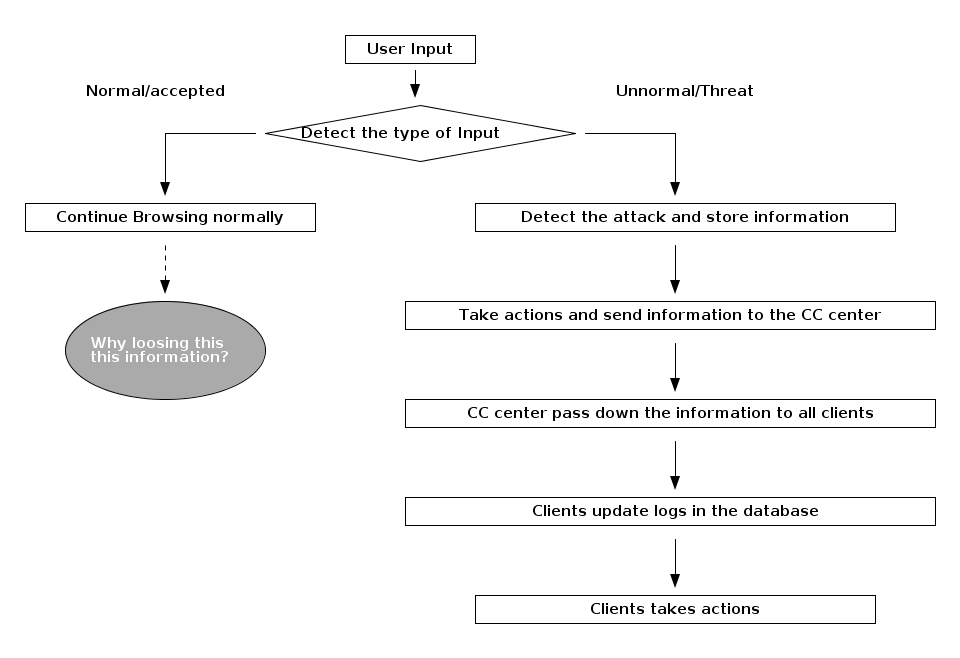
\includegraphics[width=15cm]{waf_mana}
    \caption{Zentrale Übermittlung von Angriffsdaten nach~\cite{Manaseer2018}}
    \label{fig.wafmana}
  \end{center}
\end{figure}

% Oder: Der xxx Algorithmus

% Oder: Der yyy Algorithmus

% Zusammenfassung: ca. 0,5 Seiten
\section{Zusammenfassung}

Nach der kurzen zeitlichen Einordnung über die Entstehung anomaliebasierter Web Application Firewalls im vorherigen Kapitel lieferte dieses Kapitel einen Einblick in einen Teil der bestehenden Daten. Dazu wurde der Umfang und Inhalt des 2010 von Carmen Torrano-Giménez erstellten Datensatzes \emph{CSIC2010} näher betrachtet. Es wurden einige Modernisierungsmaßnahmen vorgeschlagen, die dem veralteten Datensatz zu etwas mehr Allgemeingültigkeit und vor allem Genauigkeit verhelfen.\\

Das nächste Kapitel betrachtet die praktische Umsetzung der angedachten Ziele. Es soll dargestellt werden, wie ein neuer Datensatz generiert bzw. der bestehende Daten erweitert werden und wie neue Daten gesammelt werden können. 

\begin{neu}
  Anfang mit Aufnahme des Altenbestands, hinzufügen Entwicklungsumgebung, Test, etc

  Entwicklung Zentrale Steuerung

  Entwicklung ML Anteil
\end{neu}